\documentclass[a4paper,12pt]{article}

\usepackage[margin=2cm]{geometry}

\usepackage{graphicx}

% For cross-referencing
\usepackage{xr}
\externaldocument{main_plos}
\externaldocument[S1.]{S1_Text}
\externaldocument[S2.]{S2_Text}
\externaldocument[S3.]{S3_Text}
\externaldocument[S4.]{S4_Text}


% Caption package for small captions option
% ... convenient to list figures during manuscript processing
\usepackage{caption}
% Language and fonts
\usepackage[english]{babel}
\usepackage[T1]{fontenc}
\usepackage[utf8]{inputenc}

% Math Stuff
\usepackage{amsmath,amsfonts}
\newcommand{\argmax}{\operatornamewithlimits{argmax}}
\newtheorem{theorem}{Theorem}

% Chemical Stuff
\usepackage[version=3]{mhchem}

\usepackage{hyperref}
% Add an S4
\renewcommand{\thetable}{S4.\arabic{table}}%
\renewcommand{\thefigure}{S4.\arabic{figure}}%
\renewcommand{\theequation}{S4.\arabic{equation}}
\renewcommand{\thesection}{S4.\arabic{section}}%

\usepackage{color} 
\newcommand{\tr}[1]{{#1}}

\begin{document}
\begin{flushleft}
{\Large
\textbf\newline{\textbf{S4 Text -- Kinetic model of the ppGpp system in \textit{Escherichia coli}\footnote{Supporting Information of "Dynamical Allocation of Cellular Resources as an Optimal Control Problem: Novel Insights into Microbial Growth Strategies"}}}
}
\newline
% Insert author names, affiliations and corresponding author email (do not include titles, positions, or degrees).
\\
Nils Giordano \textsuperscript{1,3},
Francis Mairet \textsuperscript{2},
Jean-Luc Gouzé \textsuperscript{2},
Johannes Geiselmann \textsuperscript{1,3,*},
Hidde de Jong \textsuperscript{3,*}
\\
\bigskip
\bf{1} Université Grenoble Alpes, Laboratoire Interdisciplinaire de Physique (CNRS UMR 5588), 140 rue de la Physique BP 87, 38402 Saint Martin d'Hères, France
\\
\bf{2} Inria, Sophia-Antipolis Méditerranée research centre, 2004 route des Lucioles, BP 93, 06902 Sophia-Antipolis Cedex, France
\\
\bf{3} Inria, Grenoble - Rhône-Alpes research centre, 655 avenue de l'Europe, Montbonnot, 38334 Saint Ismier Cedex, France
\\
\bigskip

* Corresponding authors with equal contributions:\\
Hidde.de-Jong@inria.fr, Hans.Geiselmann@ujf-grenoble.fr
\end{flushleft}

The recently published model of Bosdriesz \textit{et al.}~\cite{bosdriesz_how_2015} provides a synthesis of the currently available knowledge of the ppGpp regulatory system.
\tr{Through the mechanisms of ppGpp production and degradation, it describes regulation of the synthesis of ribosomal RNA.}
We explain below how we use the model to compare the action of the ppGpp system with the on-off control strategy.
The denomination of variables and parameters follows the Supporting Information of~\cite{bosdriesz_how_2015} \tr{, and is reproduced in Table~\ref{S4.tab:notations} in order to make the text self-contained.}

\tr{The evolution of the cellular concentration of ppGpp is described in~\cite{bosdriesz_how_2015} by}
\begin{equation}
\label{eq:ppGpp}
\frac{d\texttt{ppGpp}}{dt} = v_{RelA}(r_{t,tot}) + v_{spoT} - k_{spoT} \cdot \texttt{ppGpp},
\end{equation}
\tr{where $v_{spoT}$ and $k_{spoT}$ are constants (see Table~\ref{S4.tab:notations}), and $v_{RelA}$ is a function of $r_{t,tot}$, the total concentration of "stalled" ribosomes:} 
\begin{equation}
\label{eq:vrelA}
v_{RelA}(r_{t,tot}) = k_{RelA} \cdot RelA_{tot} \cdot \frac{r_{t,tot}}{K_{D,RelA} + r_{t,tot}}.
\end{equation}
\tr{The amount of stalled ribosomes is determined by the equilibrium between charged and uncharged tRNA, $t_{ai}$ and $t_{i}$, in the cell:}
\begin{equation}
\label{eq:rttot}
r_{t,tot} = \sum_i r_{ti} = \sum_i r_i \frac{t_i/\kappa_{t}}{1+t_{ai}/\kappa_{ta}+t_i/\kappa_{t}},
\end{equation}
\tr{which can be rewritten as
\begin{equation}
\label{eq:rttot-f}
r_{t,tot} = \sum_i r_i \frac{t_i/\kappa_{t}}{1+(0.5 r-t_i)/\kappa_{ta}+t_i/\kappa_{t}},
\end{equation}
using the assumption that $t_{tot,i}  = t_{ai} + t_i = 0.5 \cdot r$.
$r_i$ denotes the concentration of ribosomes recognizing amino acid  $i$.
Finally, with $r = \sum_i r_i$ the total ribosome concentration and $a_i$ the concentration of amino acid $i$, the dynamics of the charged tRNA concentration is described by
\begin{equation}
\label{eq:ti_dynamic}
\frac{dt_{ai}}{dt} = v_{tai}(a_i, t_{i}) - f_i \cdot v_{ribosome}(t_i,r),
\end{equation}
with $v_{tai}(a_i, t_{i})$ the synthesis rate of charged tRNA, and $f_i \cdot v_{ribosome}(t_i,r)$ their consumption via protein synthesis.
In particular,
\begin{eqnarray}
v_{tai}(a_i, t_{i}) &=& k_{Si} \cdot S_{tot,i} \cdot \frac{t_i\, a_i}{t_i\,  K_{Mai} + a_i\,  K_{Mti} + t_i\,  a_i}, \label{eq:vtai}\\
v_{ribosome}(t_i, r) &=& k_{rib} \cdot r \cdot \left(1+ \sum_i \left[ f_i \cdot \left( 1 + \frac{t_i}{\kappa_t} \right) \frac{\kappa_{ta}}{0.5\cdot r - t_i} \right]\right)^{-1}. \label{eq:vrib}
\end{eqnarray}

For comparison with our framework, we need $\texttt{ppGpp}$ as a direct function of the total amino acid concentration $a = \sum_i a_i$ (a proxy for precursors) and total ribosome concentration $r$ (a proxy for gene expression machinery).
To this end, we made two additionnal assumptions}:
\begin{description}
\item[(A1)] All concentrations specific to one type of amino acid $i$ ($a_i$, $t_{ai}$, $t_{i}$, $r_i$) are in the same proportion $f_i = f = 1/20$ with respect to the total concentrations ($a$, $t_{a}$, $t$, $r$).
\item[(A2)] We apply a quasi-steady-state approximation (QSSA) to the dynamics of the concentration of the charged tRNAs ($t_{ai}$) and the concentration of ppGpp ($\texttt{ppGpp}$).
That is, the dynamics of these variables are assumed fast relative to the dynamics of the amino acid concentrations ($a_i$) and the total ribosome concentration ($r$).
\end{description}
\tr{Using (A2), we can rewrite Eq.~\ref{eq:ti_dynamic} as follow:
\begin{equation}\label{eq:vtai_vrib}
v_{tai}(a_i, t_{i}) = f_i \cdot v_{ribosome}(t_i,r),
\end{equation}
which, using (A1) and Eqs~\ref{eq:vtai} and \ref{eq:vrib}, leads to:
\begin{equation}
\label{eq:vtai_vrib_without_sum}
k_{Si} \cdot S_{tot,i} \cdot \frac{t_i\, a_i}{t_i\, K_{Mai} + a_i\, K_{Mti} + t_i\, a_i}
= f_i \cdot k_{rib} \cdot r \cdot
  \left(1 + \frac{\kappa_{ta}}{0.5 r - t_i} \cdot \left( 1 + \frac{t_i}{\kappa_t} \right)  \right)^{-1}.
\end{equation}
By rearranging both sides of the equation, $t_i$ can be expressed as a function of $a_i$ and $r$, which yields:}

\begin{equation}
\begin{alignedat}{2}
&A {t_i}^2 + B t_i + C = 0, \;\;\; \text{with}\\
&A = \frac{k_{Si} \,S_{tot,i} \,a_i}{f_i\, k_{rib} \,r} \left( \frac{\kappa_{ta}}{\kappa_t} - 1\right) + K_{Mai} + a_i,\\
&B = \frac{k_{Si} \,S_{tot,i} \,a_i}{f_i \,k_{rib} \,r} (0.5\,r+\kappa_{ta}) + a_i \,K_{Mti} - 0.5\,r\,(K_{Mai} + a_i),\\
&C = - 0.5 \,r \,a_i \,K_{Mti},
\end{alignedat}
\end{equation}
and therefore
\[
t_i (a_i, r) = \frac{-B \pm \sqrt{B^2 - 4AC}}{2A}.
\]
It is not difficult to show that the only solution on $[0, 0.5\,r]$ is
\begin{equation}
\label{eq:ti_final}
t_i (a_i, r) = \frac{-B + \sqrt{B^2 - 4AC}}{2A}.
\end{equation}
\tr{
From this result, we obtain $r_{t,tot}$ as a function of $a_i$ and $r$, by applying (A1) to Eq.~\ref{S4.eq:rttot-f}:
\begin{equation}
\label{eq:rttot-f_without_sum}
r_{t,tot}(t_i, r) = r \cdot \frac{t_i/\kappa_{t}}{1+(0.5 r-t_i)/\kappa_{ta}+t_i/\kappa_{t}},
\end{equation}
and substituting $t_i$ by the expression of Eq.~\ref{eq:ti_final}.

Finally, we apply (A2) to Eq.~\ref{eq:ppGpp} and obtain the final expression giving the concentration of ppGpp as a function of the total amino acid and ribosome concentrations:
\begin{equation}
\texttt{ppGpp}(a_i, r) = \frac{1}{k_{spoT}} \left( k_{RelA} \cdot RelA_{tot} \cdot \frac{r_{t,tot}(a_i, r)}{K_{D,RelA} + r_{t,tot}(a_i,r)} + v_{spoT} \right).
\end{equation}
}
This function is represented in Fig.~\ref{S4.fig:ppGpp} with parameters taken from Table~\ref{tab:notations}.

The plotted surface of the function resembles the inverse of the on-off control strategy in Fig.~\ref{fig:ppGppsurface}, as expected, bearing in mind that ppGpp has an inhibitory effect on the synthesis of ribosomal RNA.
We assumed a Michaelis-Menten inhibition for the regulatory effect of ppGpp on rRNA synthesis, and thus indirectly on the synthesis of ribosomal proteins~\cite{potrykus_pppgpp_2008,keener_regulation_1996}:
\begin{equation}
\alpha (\texttt{ppGpp}) = \frac{K_I}{K_I + \texttt{ppGpp}}.
\end{equation}
The inhibitory constant $K_I$ lies in the dynamical range of variation of $\texttt{ppGpp}$.
In Fig.~\ref{fig:ppGppsurface} in the main text, we took $K_I = 10$~$\mu$M.

\bibliographystyle{plos2015}
\bibliography{references}

\pagebreak
\begin{figure}[!ht]
\centering
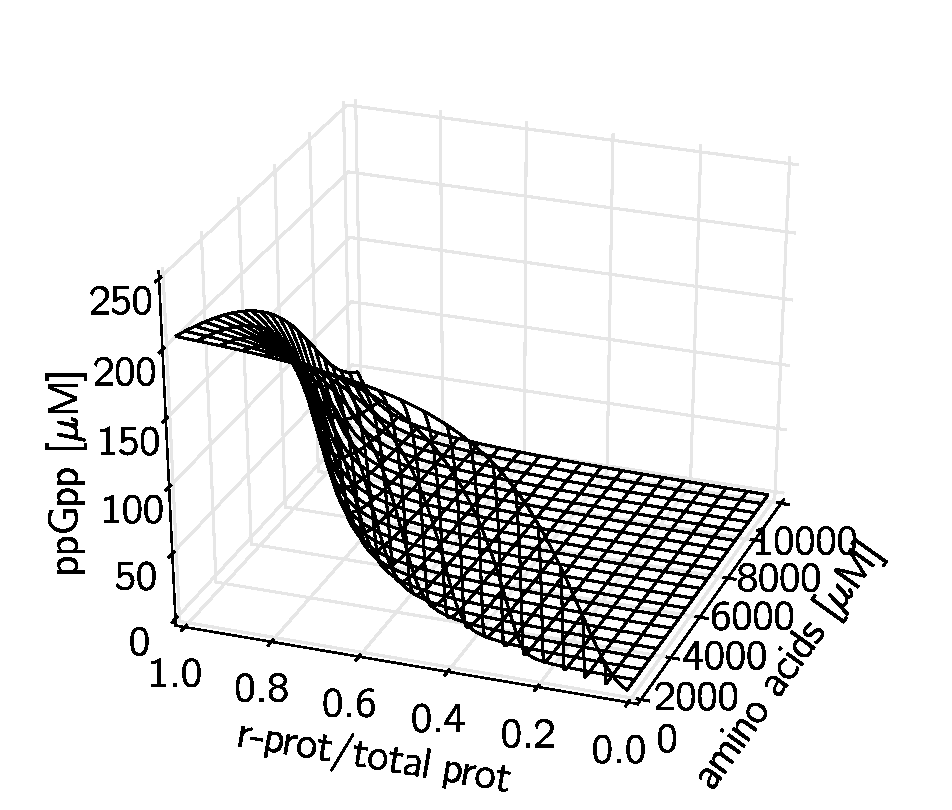
\includegraphics[width=0.7\textwidth]{./Fig/FigS4-1.eps}
\caption[ppGpp concentration is a function of total ribosome and amino acid concentrations.]
{
{\bf ppGpp concentration is a function of total ribosome and amino acid concentrations.}\newline
We assume the dynamics of ppGpp to be fast on the time-scale of changes in the ribosome and amino acid concentrations.
The concentration of ppGpp can thus be expressed as a function of the latter two variables, using the model of Bosdriesz \textit{et al.}~\cite{bosdriesz_how_2015}.
Parameters are taken from Table~\ref{tab:notations}.
}
\label{fig:ppGpp}
\end{figure}

\pagebreak

\begin{table}[!h]
\centering
\tr{
\begin{tabular}{cccl}
\hline
\hline
\textbf{Symbol} & \textbf{Value} & \textbf{Unit} & \textbf{Description} \\
\hline
\hline
$a_i$ & -- & $\mu$M & Concentration of aa $i$ (not incorporated in protein)\\

$t_{ai}$ & -- & $\mu$M & Concentration of tRNA charged with aa $i$\\

$t_{i}$ & -- & $\mu$M & Concentration of free tRNA conjugate to aa $i$\\

$t_{tot,i}$ &  $0.5 \cdot r$ & $\mu$M & Total concentration of tRNA conjugate to aa $i$\\

$r_{i}$ & -- & $\mu$M & Total concentration of ribosome with an A-site for aa $i$\\

$r_{ti}$ & -- & $\mu$M & Ribosomes with uncharged tRNA in an A-site for aa $i$\\

$\texttt{ppGpp}$ & -- & $\mu$M & Concentration of ppGpp\\
\hline
$a$ & $\sum_i a_{i}$ & $\mu$M & Total concentration of aa (not incorporated in protein)\\

$t_{a}$ & $\sum_i t_{ai}$ & $\mu$M & Total concentration of tRNA charged with aa\\

$t$ & $\sum_i t_{i}$ & $\mu$M & Total concentration of free tRNA\\

$r_{t,tot}$ & $\sum_i r_{ti}$ & $\mu$M & Total concentration of uncharged tRNA bound to ribosomes\\

$r$ & $\sum_i r_i$ & $\mu$M & Total concentration of ribosomes\\
\hline
$v_{RelA}$ & -- & $\mu$M/s & Rate of RelA-catalyzed ppGpp synthesis\\

$v_{SpoT}$ & $10^{-3}$ & $\mu$M/s & Rate of ppGpp synthesis by SpoT\\

$v_{tai}$ & -- & $\mu$M/s & Rate of amino-acyl tRNA $i$ synthetase\\

$v_{ribosome}$ & -- & $\mu$M/s & Total rate of protein synthesis\\
\hline
$k_{rib}$ & 20 & s\textsuperscript{-1} & $k_{cat}$ of protein elongation\\

$k_{RelA}$ & 75 & s\textsuperscript{-1} & $k_{cat}$ of ppGpp synthesis by RelA\\

$K_{D,RelA}$ & 0.26 & $\mu$M & Michaelis constant of RelA-catalyzed ppGpp production\\

$RelA_{tot}$ & 1/15 & $\mu$M & RelA concentration\\

$k_{SpoT}$ & $\ln (2) / 30$ & s\textsuperscript{-1} & Rate of ppGpp degradation by SpoT\\

$\kappa_t$ & 500 & $\mu$M & Dissociation constant of uncharged tRNA-ribosome complex\\

$\kappa_{ta}$ & 1 & $\mu$M & Dissociation constant of charged tRNA-ribosome complex\\

$k_{Si}$ & 100 & s\textsuperscript{-1} & $k_{cat}$ of aminoacyl-tRNA synthetase\\

$S_{tot,i}$ & 1 & $\mu$M & Total concentration of aminoacyl-tRNA synthetase for aa $i$\\

$K_{Mai}$ & 100 & $\mu$M & Michaelis constant of aa-tRNA synthetase for amino acids\\

$K_{Mti}$ & 1 & $\mu$M & Michaelis constant of aa-tRNA synthetase for uncharged tRNA\\

$f_i$ & 1/20 & -- & Proportion of aa $i$ in proteins (Assumption A1)\\

\end{tabular}
}
\caption{\textbf{Parameters and variables reused from Bosdriesz \textit{et al.}~\cite{bosdriesz_how_2015}}.} The abbreviation aa denotes amino acids.
\label{tab:notations}
\end{table}

\end{document}

